%%%%%%%%%%%%%%%%%%%%%%%%%%%%%%%%%%%%%%%%%
% Journal Article
% LaTeX Template
% Version 1.3 (9/9/13)
%
% This template has been downloaded from:
% http://www.LaTeXTemplates.com
%
% Original author:
% Frits Wenneker (http://www.howtotex.com)
%
% License:
% CC BY-NC-SA 3.0 (http://creativecommons.org/licenses/by-nc-sa/3.0/)
%
%%%%%%%%%%%%%%%%%%%%%%%%%%%%%%%%%%%%%%%%%

%----------------------------------------------------------------------------------------
%	PACKAGES AND OTHER DOCUMENT CONFIGURATIONS
%----------------------------------------------------------------------------------------

\documentclass{article}

%\documentclass{aastex}  % version 5.0 or prior
%\usepackage{natbib}



\usepackage{graphicx}
\usepackage{lipsum} % Package to generate dummy text throughout this template
%\usepackage[sc]{mathpazo} % Use the Palatino font
\usepackage[T1]{fontenc} % Use 8-bit encoding that has 256 glyphs
\linespread{1.05} % Line spacing - Palatino needs more space between lines
\usepackage{microtype} % Slightly tweak font spacing for aesthetics

\usepackage[margin=1in,columnsep=20pt]{geometry} % Document margins
\usepackage{multicol} % Used for the two-column layout of the document
\usepackage[hang, small,labelfont=bf,up,textfont=it,up]{caption} % Custom captions under/above floats in tables or figures
\usepackage{booktabs} % Horizontal rules in tables
\usepackage{float} % Required for tables and figures in the multi-column environment - they need to be placed in specific locations with the [H] (e.g. \begin{table}[H])
\usepackage{hyperref} % For hyperlinks in the PDF
\usepackage{subcaption}

\usepackage{lettrine} % The lettrine is the first enlarged letter at the beginning of the text
\usepackage{paralist} % Used for the compactitem environment which makes bullet points with less space between them
\usepackage{amsmath}
\usepackage{abstract} % Allows abstract customization
\renewcommand{\abstractnamefont}{\normalfont\bfseries} % Set the "Abstract" text to bold
\renewcommand{\abstracttextfont}{\normalfont\small\itshape} % Set the abstract itself to small italic text

\usepackage{titlesec} % Allows customization of titles
%\renewcommand\thesection{\Roman{section}} % Roman numerals for the sections
%\renewcommand\thesubsection{\Roman{subsection}} % Roman numerals for subsections
%\renewcommand\thesubsubsection{\Alph{subsubsection}} % Roman numerals for subsections
\titleformat{\section}[block]{\Large\scshape}{\thesection}{1em}{} % Change the look of the section titles
\titleformat{\subsection}[block]{\large}{\thesubsection}{1em}{} % Change the look of the section titles
\titleformat{\subsubsection}[block]{}{\thesubsubsection}{1em}{} % Change the look of the section titles

\usepackage{fancyhdr} % Headers and footers
\pagestyle{fancy} % All pages have headers and footers
\fancyhead{} % Blank out the default header
\fancyfoot{} % Blank out the default footer
\fancyhead[C]{Montana State University \quad $\bullet$ \quad CSCI 466 Artificial Intelligence \quad $\bullet$ \quad Group 21} % Custom header text
\fancyfoot[RO,LE]{\thepage} % Custom footer text

\newcommand{\ve}[1]{\boldsymbol{\mathbf{#1}}}

%----------------------------------------------------------------------------------------
%	TITLE SECTION
%----------------------------------------------------------------------------------------

\title{\vspace{-15mm}\fontsize{24pt}{10pt}\selectfont\textbf{CSCI 446 Artificial Intelligence \\ Project 2 Final Report} \\[-2mm]} % Article title
\date{\today}
\author{
\large
\textsc{Roy Smart} \and \textsc{Nevin Leh} \and \textsc{Brian Marsh}\\[2mm] % Your name
}


%----------------------------------------------------------------------------------------

\begin{document}

\maketitle % Insert title

\thispagestyle{fancy} % All pages have headers and footers

%\begin{abstract}
%We present a novel way of performing MOSES data inversions using a
%\end{abstract}

%----------------------------------------------------------------------------------------
%	ARTICLE CONTENTS
%----------------------------------------------------------------------------------------

%\begin{multicols}{2} % Two-column layout throughout the main article text
\normalsize

\begin{abstract}
	
\end{abstract}
\section{Introduction}

Define MLA acronym here!!!!

	In a broad sense, machine learning refers to efforts to give computers the ability to learn without explicit instructions and encompasses a wide range of problems.  Classification in the realm of machine learning is a problem that can be solved using several algorithms, but the effectiveness of the algorithm depends greatly upon the specific dataset involved.  We implemented four algorithms to attempt to classify new data points into sets based upon previous information gained through “training.”  The algorithms used are k-Nearest Neighbors, Naïve Bayes, Tree Augmented Naïve Bayes (TAN), and Iterative Dichotomiser 3 (ID3).  Additionally, each algorithm is tested with five different datasets: the Wisconsin Breast Cancer Database, the Glass Identification Database, the Iris Plants Database, the Small Soybean Database, and the 1984 United States Congressional Voting Records Database.  The effectiveness of each algorithm is measured by the metrics of precision and convergence.  

\section{Datasets}

	In this project we are asked to train our MLAs on five different datasets: the Wisconsin Breast Cancer Database, the Glass Identification Database, the Iris Plants Database, the Small Soybean Database, and the 1984 United States Congressional Voting Records Database. 
	Each dataset has a different set of challenges to our MLAs, for example, the soybean dataset is really small, the cancer database is reasonably large, and the attributes in the glass dataset are not very well correlated (as we will soon see).
	
	\subsection{Discretization}
	
		Two datasets, the iris dataset and the glass dataset have continuous values. 
		We are asked to discretize these dataset to more accurately compare the different MLAs.
		For our project, we adopted \textit{binning} as our discretization scheme.
		Binning is a simple method for discretization that defines a certain number of adjacent intervals, known as bins, and then replaces points that fall within each bin by a value representative of that bin.
		
		For the data in this report the number of bins was set to 10. In principle, the ideal number of bins in terms of MLA precision could be any integer larger than one, but through tests we found that the ideal number of bins is proportional to the number of classes in the dataset.
	
	\subsection{Cross-Validation}
	
		Cross-validation is statistical bootstrapping techinque used to estimate the generality of a statistical model using a dataset independent of the dataset used to create the model. 
		In the context fo machine learning, this means that we will partition the full datasets into training and validation datasets. 
		For this project we are asked to use the so-called $k$-fold cross validation technique, where the full dataset is partitioned into training and testing datasets through the use of \textit{folds}. 
		The folds are found by splitting the dataset into $k$ equal sized pieces, and assigning each to be a fold. 
		One fold is selected as the validation set, and the rest of the folds are assigned to the training set. 
		This process is then repeated $k$ times, where each fold is taken to be the validation set once.
	
		To further increase the accuracy of our cross-validation process, we will \textit{stratify} the folds described by $k$-fold cross-validation technique. 
		Stratification in this context means that each fold will have an equal distribution of the classes in each dataset..
		This process makes cross-validation more accurate, because it gives each MLA adequate information on each class for every training dataset.
		Without stratification, some training datasets could give a MLA zero examples of a particular class, hurting its ability to generalize.
		
		In $k$-fold cross-validation, $k$ is a free parameter that can be tuned by the user. For this project, we have selected $k = 10$, because it will allow us to perform the convergence tests discussed in Section \ref{conv} over a larger range.
	
	\subsection{Missing Values}
	
		Some of the datasets have missing values. 
		This is problematic since most of the MLA's will yield vastly different answers if some data is missing. 
		However, we note that the appearance of missing values in the voting dataset is merely an illusion, missing values in this dataset can signify a stance on a particular issue and this information should be used by our algorithms. 
		
		Since the voting set contains no missing values, the only dataset with missing values is the cancer dataset. Since there are so few missing values and since the cancer dataset is so large, we have decided to simply delete any data with missing values from the cancer dataset. Therefore, we have found that data imputation is not necessary for this project. 
	
\section{$k$-Nearest Neighbors}
	\subsection{Training}
		K-Nearest Neighbors attempts to solve the classification problem by using already-known data points with similar characteristics to make an educated guess of the class.  The training for k-Nearest Neighbors involves simply reading in all of the dataset and storing these records as points based on their values.
		\subsubsection{Constructing Probability Table}
	\subsection{Validation}
		\subsubsection{Value Distance Metric}
		\subsubsection{Determining $k$ and $p$}
\section{Naive Bayes}
	\subsection{Training}
	
		During the training phase for naive Bayes, the algorithm,
	
		\subsubsection{Constructing Probability Table}
		
			\begin{figure}[h]
				\centering
				\begin{subfigure}[b]{0.49\textwidth}
					\centering
					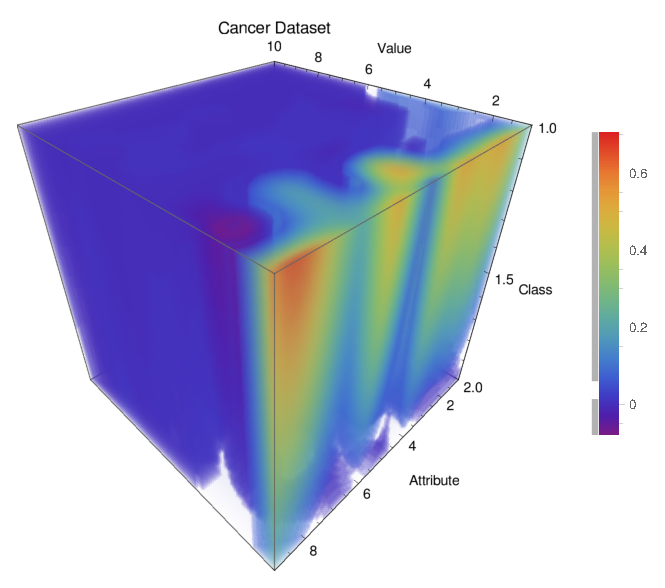
\includegraphics[width=\textwidth]{figs/NaiveBayes/plot_ptable_cancer}					
				\end{subfigure}	\	
				\begin{subfigure}[b]{0.49\textwidth}
					\centering
					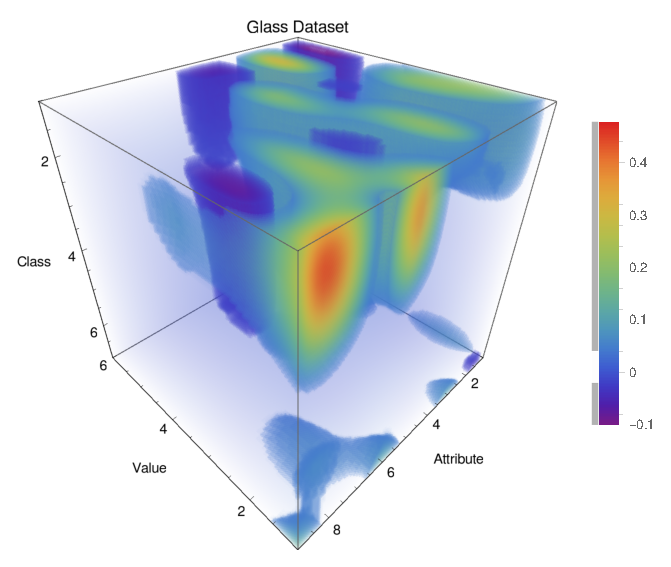
\includegraphics[width=\textwidth]{figs/NaiveBayes/plot_ptable_glass}					
				\end{subfigure} \	
				\begin{subfigure}[b]{0.49\textwidth}
					\centering
					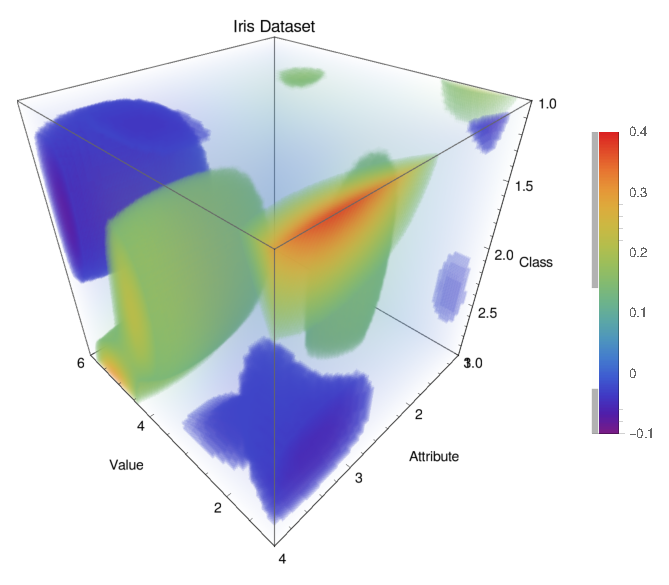
\includegraphics[width=\textwidth]{figs/NaiveBayes/plot_ptable_iris}					
				\end{subfigure} \	
				\begin{subfigure}[b]{0.49\textwidth}
					\centering
					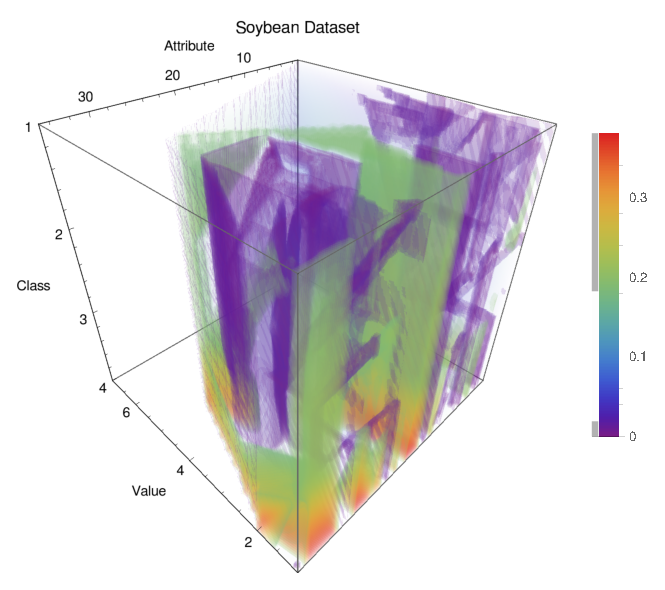
\includegraphics[width=\textwidth]{figs/NaiveBayes/plot_ptable_soybean}					
				\end{subfigure} \	
				\begin{subfigure}[b]{0.49\textwidth}
					\centering
					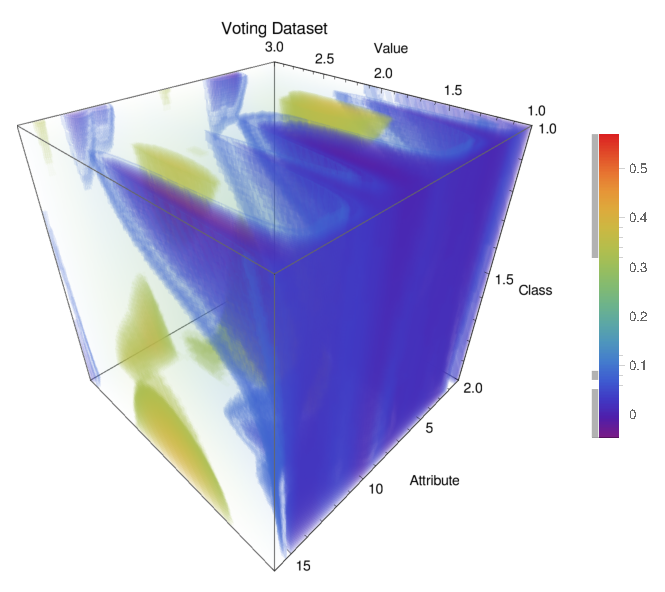
\includegraphics[width=\textwidth]{figs/NaiveBayes/plot_ptable_vote}					
				\end{subfigure}
				\caption{3D density plots of the naive Bayes probability table for all five datasets. The vertical class axis represents the value of the class, $c$, the attribute axis denotes the index of an attribute, $x$, and the value axis represents the vale of that attribute, $a$. Finally the color is equivalent to the probability of the attibute $x$ having value $a$, and the class having the value $c$}
				\label{ptable}
			\end{figure}
		
	\subsection{Validation}
		\subsubsection{Determining Class Probability Distribution}
\section{TAN}
	\subsection{Training}
		\subsubsection{Constructing Probability Table}
		\subsubsection{Constructing Augmented Tree}
	\subsection{Validation}
		\subsubsection{Determining Class Probability Distribution}
\section{ID3}
	\subsection{Training}
	\subsubsection{Tree Construction}
	The \texttt{id3} method was the main logic behind tree construction. We closely followed the decision tree learning psuedocode in Figure 18.5 in \cite{ai}. 
	ID3 is an recursive process that generates a short tree by splitting the tree one attribute at a time. 
	The first attribute to be used is the one with the most information gain. 
	Information gain can described as how much entropy the system lost by splitting on an attribute. 
	The equation for entropy is as follows:
	\begin{equation*}
	H(S) = \sum_{i=1}^{n} \left( -p_i \log_2 p_i \right). 
	\end{equation*}		
	where $p_i$ is the proportion of the number of datums in class $i$ to the total number of datums in the set $S$. 
	To use this equation the entropy of the whole system is determined first. 
	Then the sum of the entropy for each new branch is calculated and subtracted from the total entropy. We try to branch on each attribute that has not been used yet. Since the goal is to maximize this difference so the tree will be small and more general, we choose the attribute that resulted in the greatest reduction of entropy. The reduction of entropy is defined as information gain.
	The rest of the algorithm is just iterating through the tree as it is made and recursively perform the calculation on an attribute that has not been split yet. 
	The tree is finished when all leaf nodes are a single class or when attributes to split on have run out.
	In this case each leaf node that does not have a class is assigned the most common class in that leaf.
	\subsubsection{Pruning}
	We implemented reduced error pruning to help make the tree more general. The approach was to split the training set into a smaller training set and a validation set. The tree was then generated as usual using the new training set. 
	\subsection{Validation}
\section{Results}
	\subsection{Algorithm Convergence}
		\label{conv}
		\begin{figure}[h]
			\centering
			\begin{subfigure}[b]{0.49\textwidth}
				\centering
				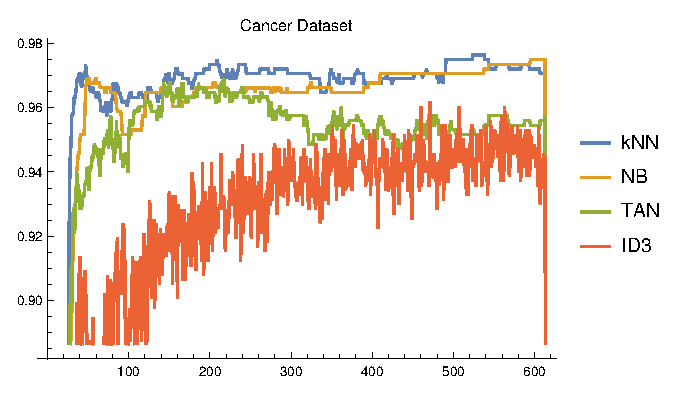
\includegraphics[width=\textwidth]{figs/plot_conv_cancer}					
			\end{subfigure}	\	
			\begin{subfigure}[b]{0.49\textwidth}
				\centering
				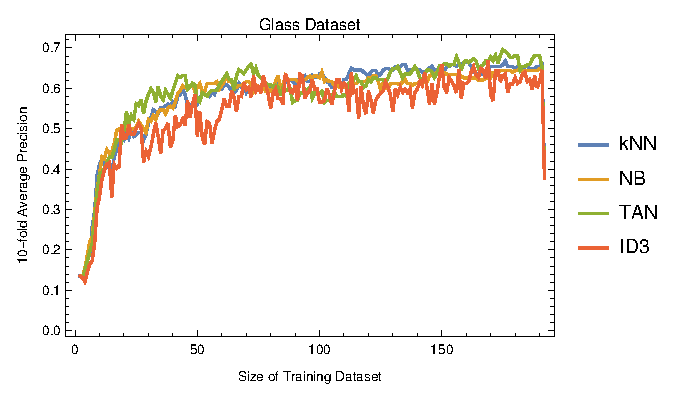
\includegraphics[width=\textwidth]{figs/plot_conv_glass}					
			\end{subfigure} \	
			\begin{subfigure}[b]{0.49\textwidth}
				\centering
				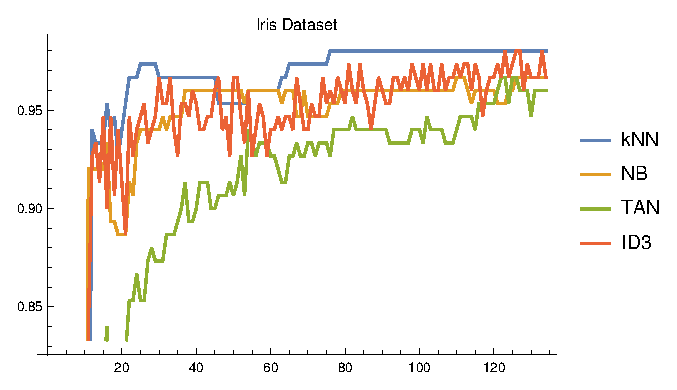
\includegraphics[width=\textwidth]{figs/plot_conv_iris}					
			\end{subfigure} \	
			\begin{subfigure}[b]{0.49\textwidth}
				\centering
				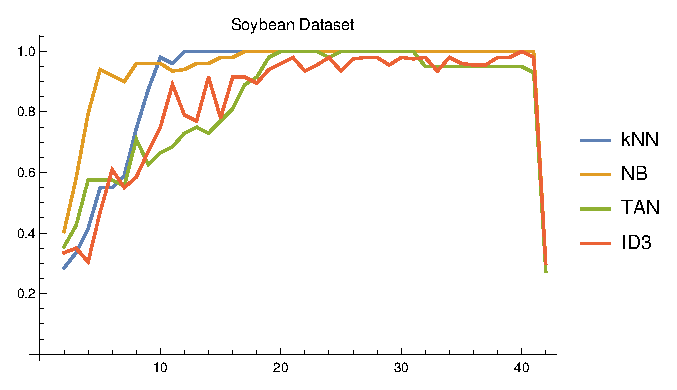
\includegraphics[width=\textwidth]{figs//plot_conv_soybean}					
			\end{subfigure} \	
			\begin{subfigure}[b]{0.49\textwidth}
				\centering
				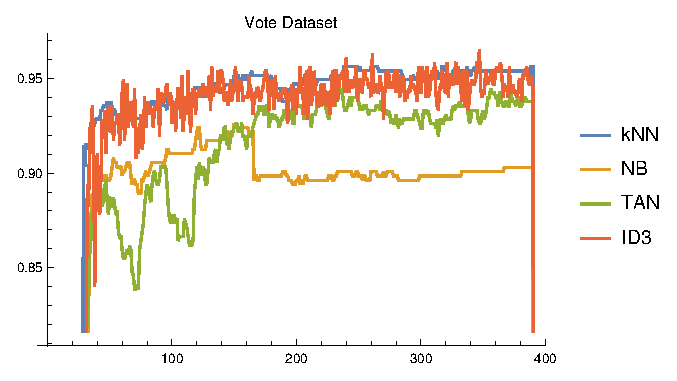
\includegraphics[width=\textwidth]{figs/plot_conv_vote}					
			\end{subfigure}
			\caption{}
			\label{conv_plot}
		\end{figure}
	\subsection{Algorithm Precision}
\section{Conclusion}
	

	\pagebreak


	%\bibliographystyle{apj}
	\bibliographystyle{apalike}
	
	\bibliography{sources}
\end{document}
